\documentclass[10pt,a4paper,oneside]{tudelft-report}
\usepackage[noabbrev]{cleveref}
\crefname{lstlisting}{listing}{listings}
\Crefname{lstlisting}{Listing}{Listings}
\usepackage{todonotes}
\presetkeys{todonotes}{inline, noline}{}
\usepackage{subcaption}
\usepackage{enumitem}
\usepackage{listings}
\usepackage{lstautogobble}
\usepackage{hhline}
\usepackage{proof}
\usepackage{natbib}
\usepackage{changes}
\usepackage{wrapfig}
\usepackage{url}
\usepackage{verbatim}
\usepackage{booktabs}
\usepackage{tikz}
\usepackage{bbding}
\usepackage{booktabs}
\usepackage{float}
\usepackage{tabularx}
\usepackage{threeparttable}
\usepackage{usebib} % Use data defined in the bib file.
\usepackage[justification=centering]{caption}
\bibinput{references}

\graphicspath{{images/}}

% \usepackage{todonotes}
\usepackage{xifthen}
% \usepackage[usenames,dvipsnames,svgnames,table]{xcolor}
\usepackage{titlesec}
\usepackage{ulem}
\newif\ifcomments

% % Disable comments by commenting the line below this one
\commentstrue

\ifcomments
% TODO's
%   \newcommand{\todo}[1]{{\color{red} TODO: #1}}
  \newcommand{\todolater}[1]{\textbf{*}}

  % maybe
  \newcommand{\maybe}[1]{{\itshape\color{orange}\{ {#1}\}}}
  \newcommand{\maybex}[1]{{\color{orange}({#1})}}

  \newcommand{\replace}[2]{{\color{red}\sout{#1}}{\color{green}#2}}
\else
  \newcommand{\todo}[1][SOMETHING]{}
  \newcommand{\todolater}[1]{}
  
  \newcommand{\maybe}[1]{}
  \newcommand{\maybex}[1]{}
  
  \newcommand{\replace}[2]{#2}
\fi

\usefont{T1}{cmr}{m}{n}

\definecolor{commentgray}{RGB}{169,173,178}
\definecolor{stringblue}{RGB}{2,48,96}
\definecolor{keywordred}{RGB}{213,60,76}
\definecolor{codedefault}{RGB}{36,41,46}

\begin{document}

% Related Work
% Problem Analysis ("4 main parts")
%       Sub problem identification
% Requirement Analysis
% Framework and Tools
% Conclusion
% \begin{titlepage}

\newcommand{\HRule}{\rule{\linewidth}{0.5mm}}

\center
 
\textsc{\LARGE Delft University of Technology}\\[1.5cm]
\textsc{\Large Bachelor Graduation Project}\\[0.5cm]
\textsc{\large Initial Research Report}\\[0.5cm]

\HRule \\[0.4cm]
{ \huge \bfseries UrbanSearch}\\[0.4cm]
\HRule \\[1.5cm]
 

\begin{minipage}{0.4\textwidth}
\begin{flushleft} \large
\emph{Authors:}\\
Tom \textsc{Brunnik}\\
Marko \textsc{Malis}\\
Gijs \textsc{Reichert}\\
Piet \textsc{van Agtmaal}\\
\end{flushleft}
\end{minipage}
~
\begin{minipage}{0.4\textwidth}
\begin{flushright} \large
\emph{Supervisor:} \\
Claudia \textsc{Hauff}

\emph{Clients:} \\
Evert \textsc{Meijers}\\
Antoine \textsc{Peris}
\end{flushright}
\end{minipage}\\[4cm]


{\large \today}\\[3cm]

\vfill

\raggedright

\includegraphics[width=0.25\textwidth]{logo}

\end{titlepage}
% \providecommand{\keywords}[1]{\textbf{Keywords:} #1}
\begin{abstract}
It is yet to be discovered how the importance of cities in the global network can be elucidated. In this paper, we develop a methodology to be able to reveal an answer to this matter. ...\\
\keywords{urban, city, data mining, document analysis, filtering}
\end{abstract}
% \newpage
% \tableofcontents
% \newpage
% This is the user manual for the UrbanSearch Web Interface. Here we will explain the different functions of the interface and how to use them. 
% \section{Related Work}
In this section we will discuss the current methods to extract relations and their strength between cities. Currently there are only two methods that are considered. The first is to manually process data from search engines. The second is to look at in what cities companies are located. After discussing these two methods we will also take a loot at NLTK \cite{nlkt_stemming}. NLTK is  a text processing tool on which (a part of) our system will be based.\\

The first currently used method is to manually process data from search engines. Researchers will input a query in a search engine (for example Google). Then they will check how many websites are found. They will also take a tiny subset of those websites, and classify them manually. There are a few problems that arise with this method. The first one is that a lot of works needs to be done by hand, which takes a lot of man-hours more then when it is done by a machine. The second is that humans are biased on what they belief is important instead of when it is automatically generated. \\

Another method that might be used is to look at companies and look at in what cities they are located. Although this might be a good indicator of the economic relations between cities, this completely ignores other relations cities might have with each other.\\

With our method we would like to process the websites through an algorithm by using the raw text from this. NLTK is a program to find relations between texts. Therefor we might base our own application on it. We would need to extend it so that we can use data from websites and so that we can visually show the data. Also although NLTK can find relations between text there are some algorithms which NLTK does not use and we might consider.

\begin{comment}
In economics there is the question "What factors play a role in economic growth?". To answer this question you would first need to give a clear definition of economic growth itself. Economic growth can be seen as a positive change in the level of goods and services produced by a city over a certain period of time. An important characteristic is that economic growth is not the same in different sectors. Economic growth can be achieved when the rate of increase in total output is greater than the rate of increase in population of a city. \\

According to Harvard University three general theories of Economic Growth within cities \cite{glaeser1992growth} are those of Marshall-Arrow-Romer (MAR) theory (1986), Porter's theory (1990) and Jacobs theory (1969). These theories focus on knowledge spillovers and claim they are most effective in cities because communication between people is more extensive. The thoeries are based on in one company improves techniquely other companies near it will also benefit. These theories differ on whether monopolies or competition benifit the growth and whether the influence is within the same industry or not (e.g. brassiere and lingerie industry). \\
Other studies focus instead on the growth of countries instead of cities. Economist Alexander Cairncross wrote that the most important factors are investment, technical process, development and trade \cite{cairncross2013factors}. Economist Stanley Fischer focusses on the influence of macroeconomics (inflation, large budged deficits, distorted foreign echange markets) \cite{fischer1993role}. Economists Rudiger Dornbusch and Alejandro Reynoso claim the most important aspects differ per region \cite{dornbusch1989financial}. \\
In other words, there are many theories and there is much research on what plays an important factor in economic growth. Although MAR's Porter's and Jacob's theory do claim one of the reason for more economic growth in cities is due to more communication between people, much research into the connectivity between cities seem to be missing. One approach that has been taken is to look at where international companies are located. This only gives limited information however. Therefore we would like to see what information can be gathered from the internet by using search engines with input consisting of 2 cities.
\end{comment}  
% \section {Requirements}

\subsection {Must haves}

\begin{enumerate}
    \item{General} 
    \begin{enumerate}
        \item Adding city names
        \item Grouping relations and “zooming” on these relations
    \end{enumerate}
    
    \item{Search Engine} 
    \begin{enumerate}
        \item Filter results
        \item Data mining
    \end{enumerate}
    
    \item{Filtering} 
    \begin{enumerate}
        \item Logic Filters 
        \item Relations Filters
    \end{enumerate}
    
    \item{Machine Learning} 
    \begin{enumerate}
        \item Types of relations
    \end{enumerate}
    
    \item{Visualization}
    \begin{enumerate}
        \item Statistics of relations? Query relations
        \item Strength of relations
        \item Types: ML CBS defined
    \end{enumerate}
\end{enumerate}


\subsection {Should haves}

\begin{enumerate}
    \item{General}
    \begin{enumerate}
        \item Pluggable datasets
    \end{enumerate}
    
    \item{Machine Learning}  
    \begin{enumerate}
        \item Generalising relations, grouping relations
    \end{enumerate}
\end{enumerate}


\subsection {Could haves}

\begin{enumerate}
    \item{General}
    \begin{enumerate}
        \item International city names
    \end{enumerate}
    
    \item{Visualization}    
    \begin{enumerate}
        \item Front end for the app
    \end{enumerate}
\end{enumerate}

\subsection {Would haves}
% \section{Frameworks and Tools}

\subsection{Extraction}
\subsubsection{Information Sources}

\paragraph{Common Crawl}
Common Crawl \cite{commoncrawl} is a freely accessible corpus of the pages across the web. Their data is updated and released on a monthly basis. Many researchers have used the data for varying purposes~\cite{smith2013dirt}~\cite{muhleisen2012web}~\cite{singh2012wikilinks}. Since the UrbanSearch project requires us to crawl the web (see section {\color{Red} FIXME}), the corpus is a very suitable candidate for us to work with.

The data of Common Crawl comes in three formats: 
\begin{itemize}
\item[WARC]
\item[WAT]
\item[WET]
\end{itemize}

For extracting data from Common Crawl, many open-source libraries are available. Common Crawls' official website refers to \texttt{cdx-index-client}\footnote{https://github.com/ikreymer/cdx-index-client} as a command line interface to their data. It allows for, among others, specifying which index to use, supports multiple output formats (plain text, \texttt{gzip} or \texttt{JSON}) and can run in parallel.

\paragraph{Eurostat}
{\color{Red} FIXME @Gijs: niet iets zeggen over wat het is?}
We identified Eurostat as a source that is not useful for the problem we're going to solve. Although Eurostat contains a lot of statistics on European cities, there is not enough useful information which contributes to giving more insight into the network connectivity of cities. Therefore, we did not include Eurostat as an information source.
\subsubsection{methods}

\subsection{Filtering and Categorizing}

\subsubsection{Clustering}
\subsubsection{Filtering}
\subsubsection{Machine Learning}
\subsubsection{TF-IDF}
basic idea: 1. using training data to assign values on words - filter meaningless words - assign words with highest value as categories? 2. Do the same on training data for each category (choose a few documents manually per category) and then check for websites for which categories has the highest value.

\subsection{Search Queries}

\subsubsection{Enter Queries}
\subsubsection{Get Results}
\subsubsection{Specifications}

\subsection{Visualisation}
\subsubsection{neo4j?}

\subsubsection{Connection between cities}
\subsubsection{The Strength of these connections}
% \newpage

\section{Code Quality}
To ensure code quality in our project we used several methods. The results from SIG \cite{sig}, a tool to ensure code quality and maintainability, are discussed and the testing is discussed.

\subsection{SIG \& BetterCodeHub}
SIG, Software Improvement Group, gives detailed insight needed to achieve better code quality and maintainability. SIG rates the code on a five star scale based on nine different values concerning code quality. Before submitting code to SIG we used BetterCodeHub\cite{better_code_hub} to check for possible faults in our code. BetterCodeHub does partly what SIG also does, but it is done online instead and can be done on every moment. Code was submitted to SIG on week 5 and week 9 of the project. Feedback can be found in appendix \ref{sig_fb}.

\subsubsection{week 5}
The first feedback from SIG was in the fifth week of development. Before uploading on BetterCodeHub our code passed all checks. For SIG it had a score from four out of five stars which means our code is above average maintainable. The last star was missed because the code is above average complex. This means that some of the functionality of some methods should be split into separate methods.
\todo{fixed this?}

\subsubsection{week 9}


\subsection{Testing}
We tested the program using three different testing methods. The first is unit testing, which tests the separate components individually. Selenium testing for testing the front-end of the app. And system testing for testing the different components together.


\subsubsection{Unit Testing}
Unit testing is done by writing automatic tests and making sure they pass every time the tests are executed. Unit tests test each method of a function separately, checking that the method does what it is supposed to do. If the method would need information from outside the class that information is mocked. This means that instead of using that other class, a fake object is made which returns a fake value. This ensures the tests will never fail due to changes in other classes. In total these test cover \todo \% of the code.

\paragraph{Selenium}
Selenium tests are automated tests that are run to test the front-end of systems. Just as normal unit testing, selenium testing is useful for regression testing.

\subsubsection{Integration tests}
Integration testing uses automated tests which test how well different components of the system work together. This is done more or less the same as unit testing, however whilst you would mock methods from other classes in unit testing, with integration testing you do not. It is assumed that the separate modules are unit tested, therefor if an error occurs it is because something is wrong with the interaction between the modules and not with the modules themselves. 

\subsubsection{System Testing}
Last we are also using system testing. System testing provides a more complete test of the entire system. This means it is useful to detect faults in the overall system, but less easy to determine where these faults may be located. System testing is done manually, which means the tests can not be easily repeated when the system changes whilst with other testing techniques this is possible. 

\subsubsection{Acceptance Testing}

% \chapter{Validation}

\section {machine learning}
To test the machine learning we will manually search for a small set of 50 pages per class. We will then manually decide to which class we would expect those pages to be sorted. Then we will run the algorithm and check whether or not a page was correctly sorted. There are 4 outcomes per page per class: true/false positives and true/false negatives. Positives are the pages that should be sorted to that class; true means they were sorted to that class, false meaning they were not sorted to that class. Negatives are pages that should not be sorted to that class and in this case true means they were indeed not sorted to that class and false means they were. So the true values are the ones that should be high. From this we can say how accurate our classifier is.

\section{unit tests}

\section{selenium tests}

\section{SIG}
SIG \cite{sig}, short for software improvement development group, is a tool to give deep code visibility we require so we can remedy current problems and prevent future vulnerabilities. A part of sig \todo{}(?) also includes betterCodeHub \cite{better_code_hub} which checks our code in 10 steps:
\begin{enumerate}
    \item \textbf {Write short units of code} \\
    Units of code should be no longer than 15 lines.
    \item \textbf {Write simple units of code} \\
    Separate units of code should contain no more than 4 branch points (if, for, while, etc)
    \item \textbf{Write code once} \\
    Shared code should be extracted, either to a new unit or to a super class
    \item \textbf{Keep unit interfaces small} \\
    The number of parameters per unit of code should be no more than four.
    \item \textbf{Separate concerns in modules} \\
    Identify and extract responsibilities of large modules to separate modules and hide implementation details behind interfaces.
    \item \textbf{Couple architecture components loosely} \\
    minimizing the amount of interface code (e.g. by using 'abstract factory' design pattern)
    \item \textbf{Keep architecture components balanced} \\
    Organize code in such a way that the number of components is between 2 and 12, and ensure the components are of approximately equal size (keep component size uniformity less than 0.71).
    \item \textbf{Keep your codebase small} \\
    Refactor existing code to achieve the same functionality using less volume, and prefer libraries and frameworks over "homegrown" implementations of standard functionality.
    \item \textbf{Automate tests} \\
    Add tests for existing code every time you change it.
    \item \textbf{Write clean code}\\
    Remove useless comments, commented code blocks, and dead code. Refactor poorly handled exceptions, magic constants, and poorly named units or variables.  
\end{enumerate}

\begin{comment}
- double city names
- city names with meaning (leiden)
- city/province names (utrecht / groningen / zeeland)
\end{comment}
% 
\chapter{Process}

\todo{fit this in somewhere}

\section{Collaboration between the team members}
The collebaration between the team members went well. The team members worked in a room in the faculty of architecture from 9-5 each day. Three of the four team members knew each other already. The work was devided even over the team members. 

\section{Collaboration between the team members and the TU Delft Coach}
Each week 9:30 on monday the team members had a meeting with the TU Delft coach. In the beginning there were some communication issues between the team and the coach but as the process went on communication became better.

\section{Collaboration between the team members and the client}
The collaboration between the team members and the client was good as well. 
Weekly meetings helped the team members making the productas good as possible to the clients wishes. 
% \newpage
\section{Implementation}
\todo{To do? To fake? To leave out? You decide!}

\subsection{Scrum}

\subsection{Implementation per week}

\subsubsection{week 1}
\subsubsection{week 2}
\subsubsection{week 3}
\subsubsection{week 4}
\subsubsection{week 5}
\subsubsection{week 6}
\subsubsection{week 7}
\subsubsection{week 8}
\subsubsection{week 9}

% \chapter{Conclusion}

\todo{ Start with "In the past few months we blah" and shortly mention the chapters
 Mention the project goal and how well it is met, without duplicating the 
 evaluation chapter}

\section{related work}
First, we discussed related work. We saw that there are currently two methods for analysing the relations between cities. Manually analysing search engine data is very slow and requires a lot of man-hours and looking at the different locations where businesses are located is only interesting for the economic relation and still misses a lot of data.
\\

\section{related work}
Second, we identified the requirements for a solution to the problem and discuss issues that might arise. The used the MoSCoW model to describe the importance of the different requirements. The most import must haves we found are being able to input place names, displaying a map with the connection data and being able to extract this data.
\\

\section{Requirement analysis}
Third, we developed a methodology for a framework that satisfies the requirements and tackles the issues. We decided to start by using data from Common Crawl, although we might later extend this to other data sources such as Delpher. After selecting relevant data (data which contains 2 or more city names) we store the data with Neo4j. We then use clustering and classifying machine learning to group the data. First we use this on all data to get the general groups (e.g. economy, health-care, immigration) and then we use this on the data per pair of cities to see what the important connection types for each city are. Then we link these connections to the general groups ('fish' might relate to economy.. etc). To visualise this data we use the graph Neo4j provides.

\section{Framework-and-tools}


\frontmatter

\lstdefinestyle{mystyle}{
    commentstyle=\color{commentgray},
    keywordstyle=\color{keywordred},
    numberstyle=\tiny\color{codedefault},
    stringstyle=\color{stringblue},
    breaklines=true,
    captionpos=b,
    frame=none,
    keepspaces=true,
    autogobble=true,
    numbers=left,
    basicstyle=\footnotesize\tudcffamily,
    numberstyle=\tudcffamily,
    numbersep=5pt,
    xleftmargin=10pt,
    showstringspaces=false
}

% Cypher query language
\lstdefinelanguage{cypher} {
  keywords={start,create,set,delete,foreach,match,%
    where,with,return,skip,limit,order,by,asc,%
    ascending,desc,descending},
  morekeywords = {[2]type,id,length,nodes,rels,%
    relationships,abs,round,sqrt,sign,head,last,%
    tail,replace,left,right,substring,lower,upper,%
    ltrim,rtrim,trim,str,shortestpath,range,count,%
    sum,min,max,avg,collect,percentile\_cont,%
    percentile\_disc},
  sensitive = false,
  morecomment=[l]{//},
  morestring=[b]",
  morestring=[b]'
}
 
\lstset{style=mystyle}
% image of UI?
\begin{titlepage}

\newcommand{\HRule}{\rule{\linewidth}{0.5mm}}

\center
 
\textsc{\LARGE Delft University of Technology}\\[1.5cm]
\textsc{\Large Bachelor Graduation Project}\\[0.5cm]
\textsc{\large Initial Research Report}\\[0.5cm]

\HRule \\[0.4cm]
{ \huge \bfseries UrbanSearch}\\[0.4cm]
\HRule \\[1.5cm]
 

\begin{minipage}{0.4\textwidth}
\begin{flushleft} \large
\emph{Authors:}\\
Tom \textsc{Brunnik}\\
Marko \textsc{Malis}\\
Gijs \textsc{Reichert}\\
Piet \textsc{van Agtmaal}\\
\end{flushleft}
\end{minipage}
~
\begin{minipage}{0.4\textwidth}
\begin{flushright} \large
\emph{Supervisor:} \\
Claudia \textsc{Hauff}

\emph{Clients:} \\
Evert \textsc{Meijers}\\
Antoine \textsc{Peris}
\end{flushright}
\end{minipage}\\[4cm]


{\large \today}\\[3cm]

\vfill

\raggedright

\includegraphics[width=0.25\textwidth]{logo}

\end{titlepage}

\mainmatter

% Three parts: background, methodology and structure
\chapter{User Manual}
This is the user manual for the UrbanSearch Web Interface. Here the different functions of the interface are explained and how to use them. 

\section{Accessing the Web Interface}
The URL "http://citynetworks.bk.tudelft.nl/" can be used to access the UrbanSearch program. After entering this URL a screen should be displayed with a menu on the left of the page, and a map on the right. After a few seconds of loading, the map on the right will display a number of cities based on the initial settings. 


\section{The Menu}
The menu on the left of the screen displays three different sections. The first section displays an option to export the data. The second section can be used to determine what cities should be displayed on the map. The last section displays the different relation types. The thresholds cities should have for each type can be adjusted here. This section also includes an option to select other weighting models that can be used.


\subsection{Exporting Data}
The first section on the menu is an export option. Here a button is displayed which can be used to export all relations between cities in an excel file (CSV). Above this button is a field in which a probably threshold can be set for the export. 

\begin{figure}[H]
    \centering
    
\includegraphics{export}
    \caption{Export}
    \label{fig:infoflow}
\end{figure}



\subsection{Selecting Cities}
The second section of the menu displays options for selecting which cities should be displayed on the map. A slider can be used to select a minimum and maximum population size for displayed cities. Underneath is a dropdown menu in which cities can be removed and added to the map manually. 

\begin{figure}[H]
    \centering
    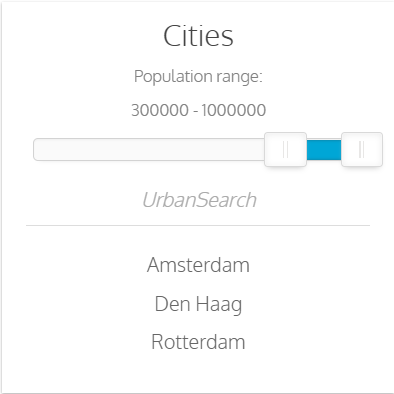
\includegraphics[scale=.74]{cities}
    \caption{Cities options}
    \label{fig:infoflow}
\end{figure}


\subsection{Selecting Relations}
In the relations section of the menu a dropdown menu is displayed which is used to select how the weights of the relations should be calculated. The standard way is to just select the occurrences of documents per relation type. However it is also possible to use a gravity model, which takes the population and the distance between cities into account. \todo{can we do this?} Beneath that are sliders for the different relationship types. Here you can change the minimum occurrences a relation type should have per two cities before the relation is taken into account. There is also an option to turn off the relation types entirely.

\begin{figure}[H]
    \centering
    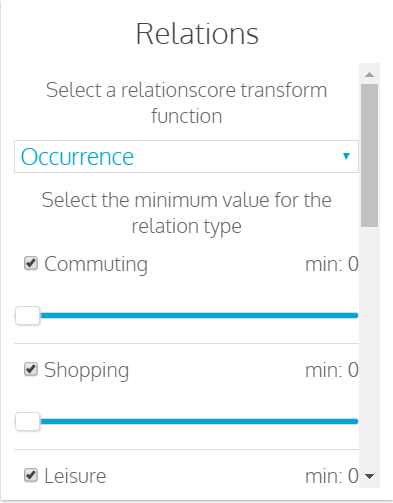
\includegraphics[scale=.74]{relations}
    \caption{Relations options}
    \label{fig:infoflow}
\end{figure}


\section{The Map}
After a few seconds needed to load the relations, a map should be displayed. This map first only contains some cities. The scroll wheel of the mouse or the plus and minus buttons in the lower right corner of the map for zooming. When hovering over a city with the mouse the population of that city will be displayed. To show the relations of a city, that city can be clicked on. The cities showing relations will have a slightly darker color than cities that have not been clicked on. You can also click on a relation. This will open up an extra window in the menu containing information about that relation.

\begin{figure}[H]
    \centering
    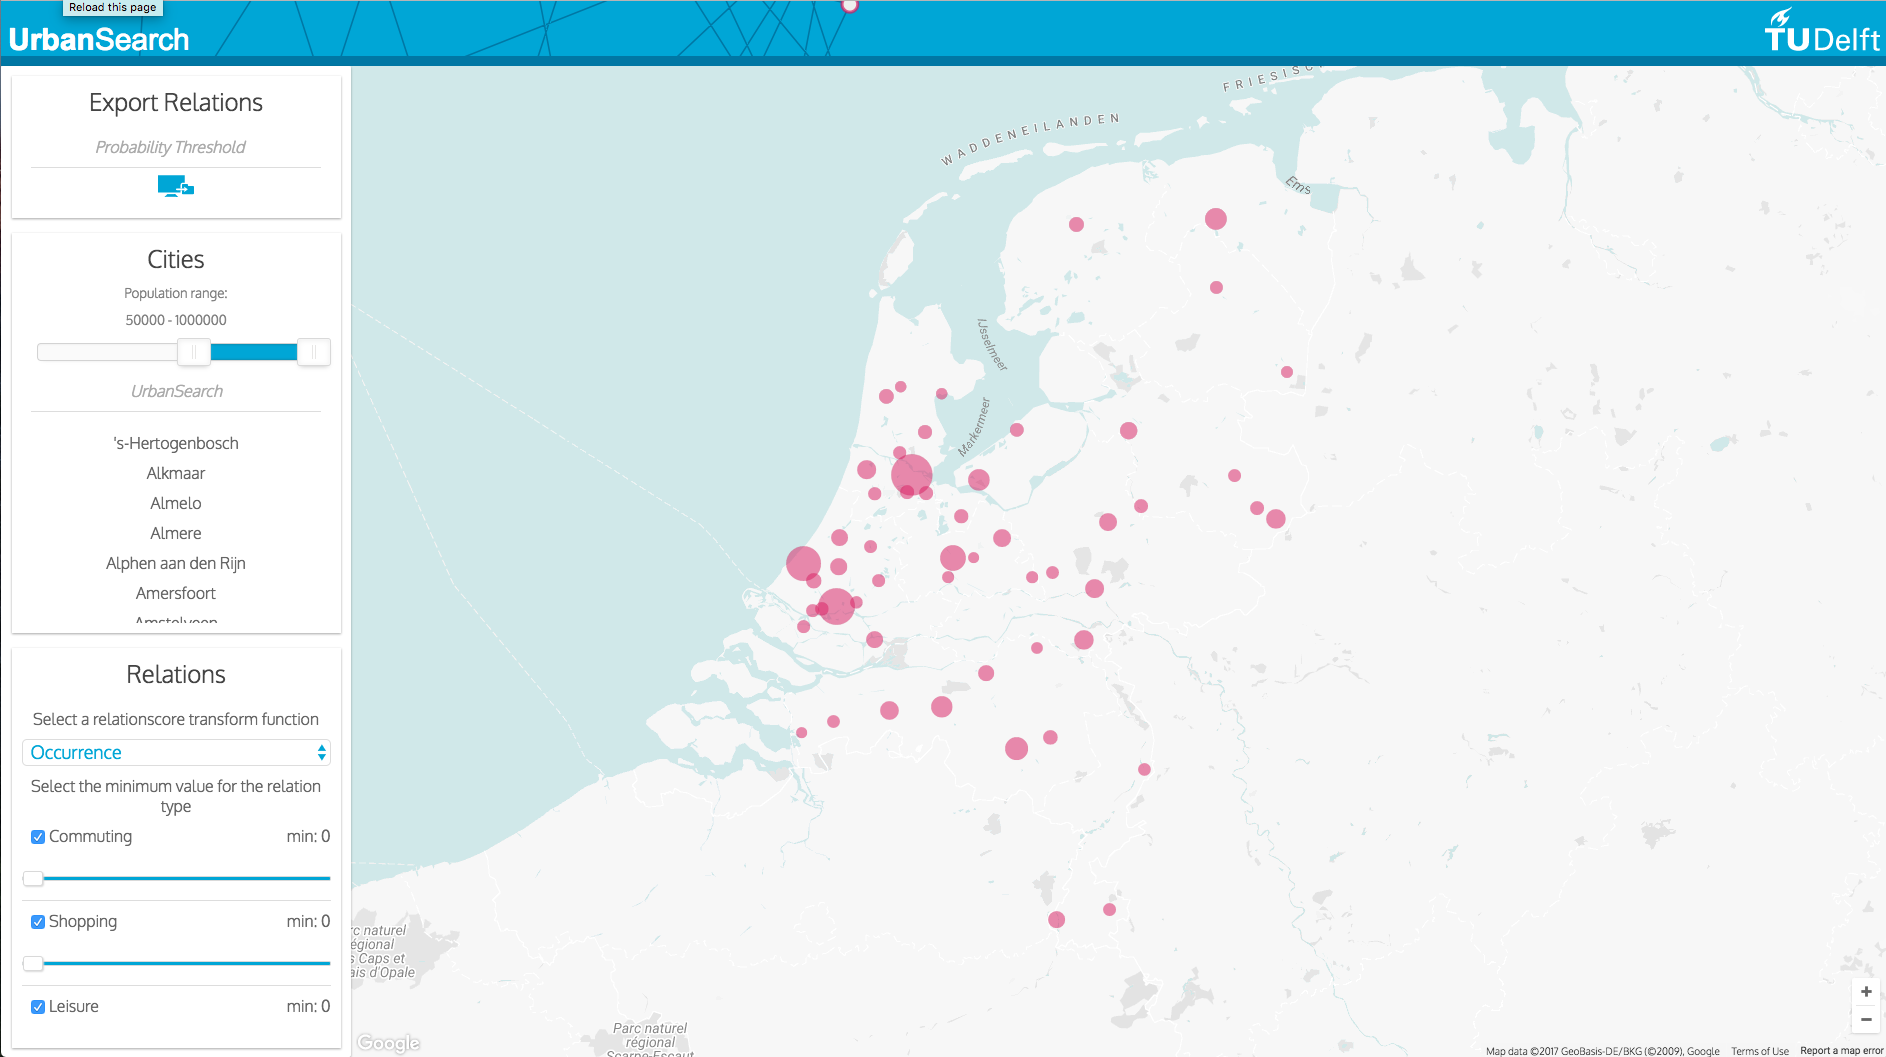
\includegraphics[scale=.5]{map}
    \caption{Map}
    \label{fig:infoflow}
\end{figure}


\begin{figure}[H]
\centering
\begin{subfigure}{.5\textwidth}
  \centering
  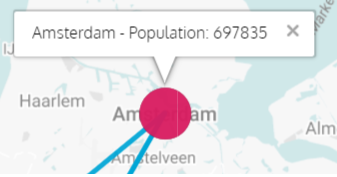
\includegraphics[width=.8\linewidth]{hover}
  \caption{Hovering over a city}
  \label{fig:sub1}
\end{subfigure}%
\begin{subfigure}{.5\textwidth}
  \centering
  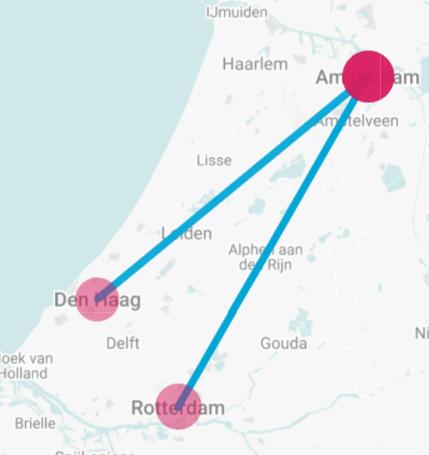
\includegraphics[width=.8\linewidth]{click}
  \caption{City showing relations}
  \label{fig:sub2}
\end{subfigure}
\label{fig:test}
\end{figure}


\subsection{Relation window}
When clicking on a relation an extra window in the menu will be opened. This contains all information about the relation between the two cities. The strength of the relations (amount of documents found for the relation between those cities) will be displayed, as well as the strength of the relations per relation type (such as commuting, shopping, leisure, ..). To check how these relationships were found the option on the lower end of this window  can be used to open up another window displaying all documents that connect those two cities.

\begin{figure}[H]
    \centering
    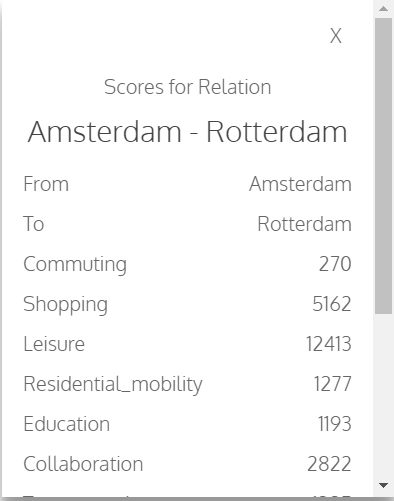
\includegraphics[scale=.7]{Score}
    \caption{Relations scores between two cities}
    \label{fig:infoflow}
\end{figure}


\subsection{Documents connecting two cities menu}
In this new window all documents will be displayed. For each document the type of relation to which the document fits and the probability this documents fits to that relation is displayed. If a document does not fit to the relation types (and is thus labelled other), it is not displayed here. The documents can be downloaded in a text file by clicking on them.

\begin{figure}[H]
    \centering
    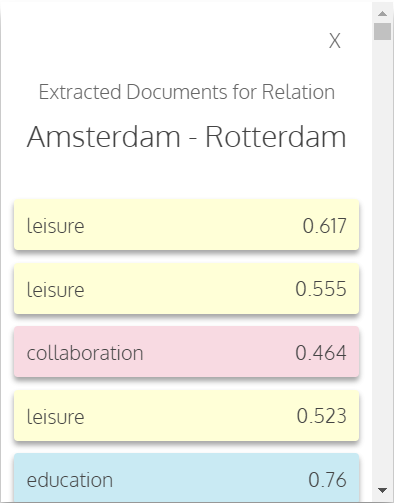
\includegraphics[scale=.7]{documents}
    \caption{Documents included in relations}
    \label{fig:infoflow}
\end{figure}



\end{document}
